\documentclass{standalone}
\usepackage{tikz}
\usetikzlibrary{patterns, positioning}

\begin{document}
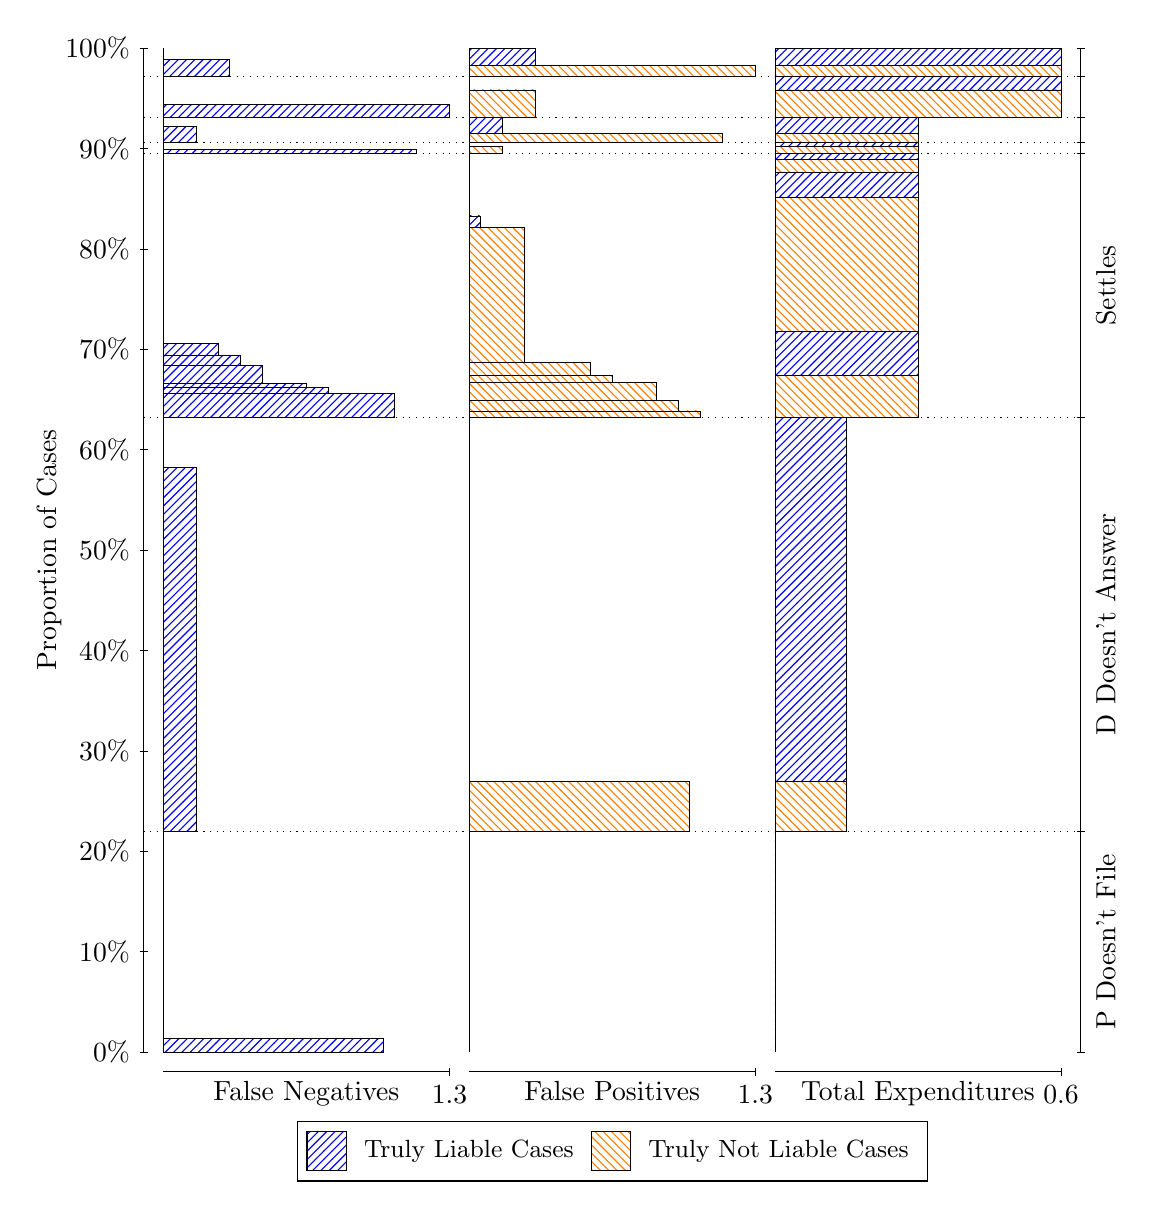
\begin{tikzpicture}
\draw[black, very thin] (1.5,1.75) -- (1.5,14.5);
\node[rotate=90, anchor=center] at (0.3, 8.125) {Proportion of Cases};
\draw[black, very thin] (1.45,1.75) -- (1.55,1.75);
\node[anchor=east] at (1.45, 1.75) {0\%};
\draw[black, very thin] (1.45,3.025) -- (1.55,3.025);
\node[anchor=east] at (1.45, 3.025) {10\%};
\draw[black, very thin] (1.45,4.3) -- (1.55,4.3);
\node[anchor=east] at (1.45, 4.3) {20\%};
\draw[black, very thin] (1.45,5.575) -- (1.55,5.575);
\node[anchor=east] at (1.45, 5.575) {30\%};
\draw[black, very thin] (1.45,6.85) -- (1.55,6.85);
\node[anchor=east] at (1.45, 6.85) {40\%};
\draw[black, very thin] (1.45,8.125) -- (1.55,8.125);
\node[anchor=east] at (1.45, 8.125) {50\%};
\draw[black, very thin] (1.45,9.4) -- (1.55,9.4);
\node[anchor=east] at (1.45, 9.4) {60\%};
\draw[black, very thin] (1.45,10.675) -- (1.55,10.675);
\node[anchor=east] at (1.45, 10.675) {70\%};
\draw[black, very thin] (1.45,11.95) -- (1.55,11.95);
\node[anchor=east] at (1.45, 11.95) {80\%};
\draw[black, very thin] (1.45,13.225) -- (1.55,13.225);
\node[anchor=east] at (1.45, 13.225) {90\%};
\draw[black, very thin] (1.45,14.5) -- (1.55,14.5);
\node[anchor=east] at (1.45, 14.5) {100\%};

\draw[black, very thin] (13.4,1.75) -- (13.4,14.5);
\draw[black, very thin] (13.35,1.75) -- (13.45,1.75);
\node[anchor=west] at (13.35, 1.75) {};
\draw[black, very thin] (13.35,4.5525) -- (13.45,4.5525);
\node[anchor=west] at (13.35, 4.5525) {};
\draw[black, very thin] (13.35,9.8098) -- (13.45,9.8098);
\node[anchor=west] at (13.35, 9.8098) {};
\draw[black, very thin] (13.35,13.159) -- (13.45,13.159);
\node[anchor=west] at (13.35, 13.159) {};
\draw[black, very thin] (13.35,13.303) -- (13.45,13.303);
\node[anchor=west] at (13.35, 13.303) {};
\draw[black, very thin] (13.35,13.616) -- (13.45,13.616);
\node[anchor=west] at (13.35, 13.616) {};
\draw[black, very thin] (13.35,14.138) -- (13.45,14.138);
\node[anchor=west] at (13.35, 14.138) {};
\draw[black, very thin] (13.35,14.5) -- (13.45,14.5);
\node[anchor=west] at (13.35, 14.5) {};

\draw[black, very thin, pattern color=blue, pattern=north east lines] (1.75,1.75) rectangle (4.5449,1.9243);
\draw[black, very thin, pattern color=orange, pattern=north west lines] (1.75,1.9243) rectangle (1.75,4.5525);
\draw[black, very thin, pattern color=blue, pattern=north east lines] (1.75,4.5525) rectangle (2.1692,9.1786);
\draw[black, very thin, pattern color=orange, pattern=north west lines] (1.75,9.1786) rectangle (1.75,9.8098);
\draw[black, very thin, pattern color=blue, pattern=north east lines] (1.75,9.8098) rectangle (4.6846,10.116);
\draw[black, very thin, pattern color=blue, pattern=north east lines] (1.75,10.116) rectangle (3.8462,10.195);
\draw[black, very thin, pattern color=blue, pattern=north east lines] (1.75,10.195) rectangle (3.5667,10.24);
\draw[black, very thin, pattern color=blue, pattern=north east lines] (1.75,10.24) rectangle (3.0077,10.469);
\draw[black, very thin, pattern color=blue, pattern=north east lines] (1.75,10.469) rectangle (2.7282,10.6);
\draw[black, very thin, pattern color=blue, pattern=north east lines] (1.75,10.6) rectangle (2.4487,10.746);
\draw[black, very thin, pattern color=orange, pattern=north west lines] (1.75,10.746) rectangle (1.75,13.159);
\draw[black, very thin, pattern color=blue, pattern=north east lines] (1.75,13.159) rectangle (4.9641,13.211);
\draw[black, very thin, pattern color=orange, pattern=north west lines] (1.75,13.211) rectangle (1.75,13.303);
\draw[black, very thin, pattern color=blue, pattern=north east lines] (1.75,13.303) rectangle (2.1692,13.503);
\draw[black, very thin, pattern color=orange, pattern=north west lines] (1.75,13.503) rectangle (1.75,13.616);
\draw[black, very thin, pattern color=blue, pattern=north east lines] (1.75,13.616) rectangle (5.3833,13.787);
\draw[black, very thin, pattern color=orange, pattern=north west lines] (1.75,13.787) rectangle (1.75,14.138);
\draw[black, very thin, pattern color=blue, pattern=north east lines] (1.75,14.138) rectangle (2.5885,14.353);
\draw[black, very thin, pattern color=orange, pattern=north west lines] (1.75,14.353) rectangle (1.75,14.5);
\draw[black, very thin, pattern color=orange, pattern=north west lines] (5.6333,1.75) rectangle (5.6333,4.3782);
\draw[black, very thin, pattern color=blue, pattern=north east lines] (5.6333,4.3782) rectangle (5.6333,4.5525);
\draw[black, very thin, pattern color=orange, pattern=north west lines] (5.6333,4.5525) rectangle (8.4282,5.1837);
\draw[black, very thin, pattern color=blue, pattern=north east lines] (5.6333,5.1837) rectangle (5.6333,9.8098);
\draw[black, very thin, pattern color=orange, pattern=north west lines] (5.6333,9.8098) rectangle (8.5679,9.892);
\draw[black, very thin, pattern color=orange, pattern=north west lines] (5.6333,9.892) rectangle (8.2885,10.024);
\draw[black, very thin, pattern color=orange, pattern=north west lines] (5.6333,10.024) rectangle (8.009,10.252);
\draw[black, very thin, pattern color=orange, pattern=north west lines] (5.6333,10.252) rectangle (7.45,10.347);
\draw[black, very thin, pattern color=orange, pattern=north west lines] (5.6333,10.347) rectangle (7.1705,10.511);
\draw[black, very thin, pattern color=orange, pattern=north west lines] (5.6333,10.511) rectangle (6.3321,12.223);
\draw[black, very thin, pattern color=blue, pattern=north east lines] (5.6333,12.223) rectangle (5.7731,12.369);
\draw[black, very thin, pattern color=blue, pattern=north east lines] (5.6333,12.369) rectangle (5.6333,13.159);
\draw[black, very thin, pattern color=orange, pattern=north west lines] (5.6333,13.159) rectangle (6.0526,13.251);
\draw[black, very thin, pattern color=blue, pattern=north east lines] (5.6333,13.251) rectangle (5.6333,13.303);
\draw[black, very thin, pattern color=orange, pattern=north west lines] (5.6333,13.303) rectangle (8.8474,13.416);
\draw[black, very thin, pattern color=blue, pattern=north east lines] (5.6333,13.416) rectangle (6.0526,13.616);
\draw[black, very thin, pattern color=orange, pattern=north west lines] (5.6333,13.616) rectangle (6.4718,13.967);
\draw[black, very thin, pattern color=blue, pattern=north east lines] (5.6333,13.967) rectangle (5.6333,14.138);
\draw[black, very thin, pattern color=orange, pattern=north west lines] (5.6333,14.138) rectangle (9.2667,14.284);
\draw[black, very thin, pattern color=blue, pattern=north east lines] (5.6333,14.284) rectangle (6.4718,14.5);
\draw[black, very thin, pattern color=orange, pattern=north west lines] (9.5167,1.75) rectangle (9.5167,4.3782);
\draw[black, very thin, pattern color=blue, pattern=north east lines] (9.5167,4.3782) rectangle (9.5167,4.5525);
\draw[black, very thin, pattern color=orange, pattern=north west lines] (9.5167,4.5525) rectangle (10.425,5.1837);
\draw[black, very thin, pattern color=blue, pattern=north east lines] (9.5167,5.1837) rectangle (10.425,9.8098);
\draw[black, very thin, pattern color=orange, pattern=north west lines] (9.5167,9.8098) rectangle (11.333,10.347);
\draw[black, very thin, pattern color=blue, pattern=north east lines] (9.5167,10.347) rectangle (11.333,10.898);
\draw[black, very thin, pattern color=orange, pattern=north west lines] (9.5167,10.898) rectangle (11.333,12.61);
\draw[black, very thin, pattern color=blue, pattern=north east lines] (9.5167,12.61) rectangle (11.333,12.916);
\draw[black, very thin, pattern color=orange, pattern=north west lines] (9.5167,12.916) rectangle (11.333,13.081);
\draw[black, very thin, pattern color=blue, pattern=north east lines] (9.5167,13.081) rectangle (11.333,13.159);
\draw[black, very thin, pattern color=orange, pattern=north west lines] (9.5167,13.159) rectangle (11.333,13.251);
\draw[black, very thin, pattern color=blue, pattern=north east lines] (9.5167,13.251) rectangle (11.333,13.303);
\draw[black, very thin, pattern color=orange, pattern=north west lines] (9.5167,13.303) rectangle (11.333,13.416);
\draw[black, very thin, pattern color=blue, pattern=north east lines] (9.5167,13.416) rectangle (11.333,13.616);
\draw[black, very thin, pattern color=orange, pattern=north west lines] (9.5167,13.616) rectangle (13.15,13.967);
\draw[black, very thin, pattern color=blue, pattern=north east lines] (9.5167,13.967) rectangle (13.15,14.138);
\draw[black, very thin, pattern color=orange, pattern=north west lines] (9.5167,14.138) rectangle (13.15,14.284);
\draw[black, very thin, pattern color=blue, pattern=north east lines] (9.5167,14.284) rectangle (13.15,14.5);
\draw[black, dotted] (1.5,4.5525) -- (13.4,4.5525);
\draw[black, dotted] (1.5,9.8098) -- (13.4,9.8098);
\draw[black, dotted] (1.5,13.159) -- (13.4,13.159);
\draw[black, dotted] (1.5,13.303) -- (13.4,13.303);
\draw[black, dotted] (1.5,13.616) -- (13.4,13.616);
\draw[black, dotted] (1.5,14.138) -- (13.4,14.138);
\draw[black, very thin] (1.75,1.5) -- (5.3833,1.5);
\node[anchor=north] at (3.5667, 1.5) {False Negatives};
\draw[black, very thin] (5.3833,1.45) -- (5.3833,1.55);
\node[anchor=north] at (5.3833, 1.45) {1.3};

\draw[black, very thin] (5.6333,1.5) -- (9.2667,1.5);
\node[anchor=north] at (7.45, 1.5) {False Positives};
\draw[black, very thin] (9.2667,1.45) -- (9.2667,1.55);
\node[anchor=north] at (9.2667, 1.45) {1.3};

\draw[black, very thin] (9.5167,1.5) -- (13.15,1.5);
\node[anchor=north] at (11.333, 1.5) {Total Expenditures};
\draw[black, very thin] (13.15,1.45) -- (13.15,1.55);
\node[anchor=north] at (13.15, 1.45) {0.6};

\node[black, centered, rotate=90] at (13.72, 3.1512) {P Doesn't File};
\node[black, centered, rotate=90] at (13.72, 7.1811) {D Doesn't Answer};
\node[black, centered, rotate=90] at (13.72, 11.485) {Settles};





\draw (7.449999999999999,1.5) node[draw=none] (baseCoordinate) {};
\begin{scope}[align=center]
        \matrix[scale=0.5, draw=black, below=0.5cm of baseCoordinate, nodes={draw}, column sep=0.1cm]{
            \node[rectangle, draw, minimum width=0.5cm, minimum height=0.5cm, pattern=north east lines, pattern color=blue] {}; &
            \node[draw=none, font=\small] (B) {Truly Liable Cases}; &
            \node[rectangle, draw, minimum width=0.5cm, minimum height=0.5cm, pattern=north west lines, pattern color=orange] {}; &
            \node[draw=none, font=\small] (B) {Truly Not Liable Cases}; \\
            };
\end{scope}

\end{tikzpicture}
\end{document}